This is about the alphasense NO2 results.

One AlphaSense NO2 sensor was tested against the EPA reference.  It was 2 months old at the time of installation, and ran for 21 days (from 5/23 - 6/13 2016).  This test gave 30,150 minute resolved samples.


\subsection{Pre-processing}

Talk about process for taking raw aux/working electrodes and making the basic calibration data.


\begin{figure}[htb]
 	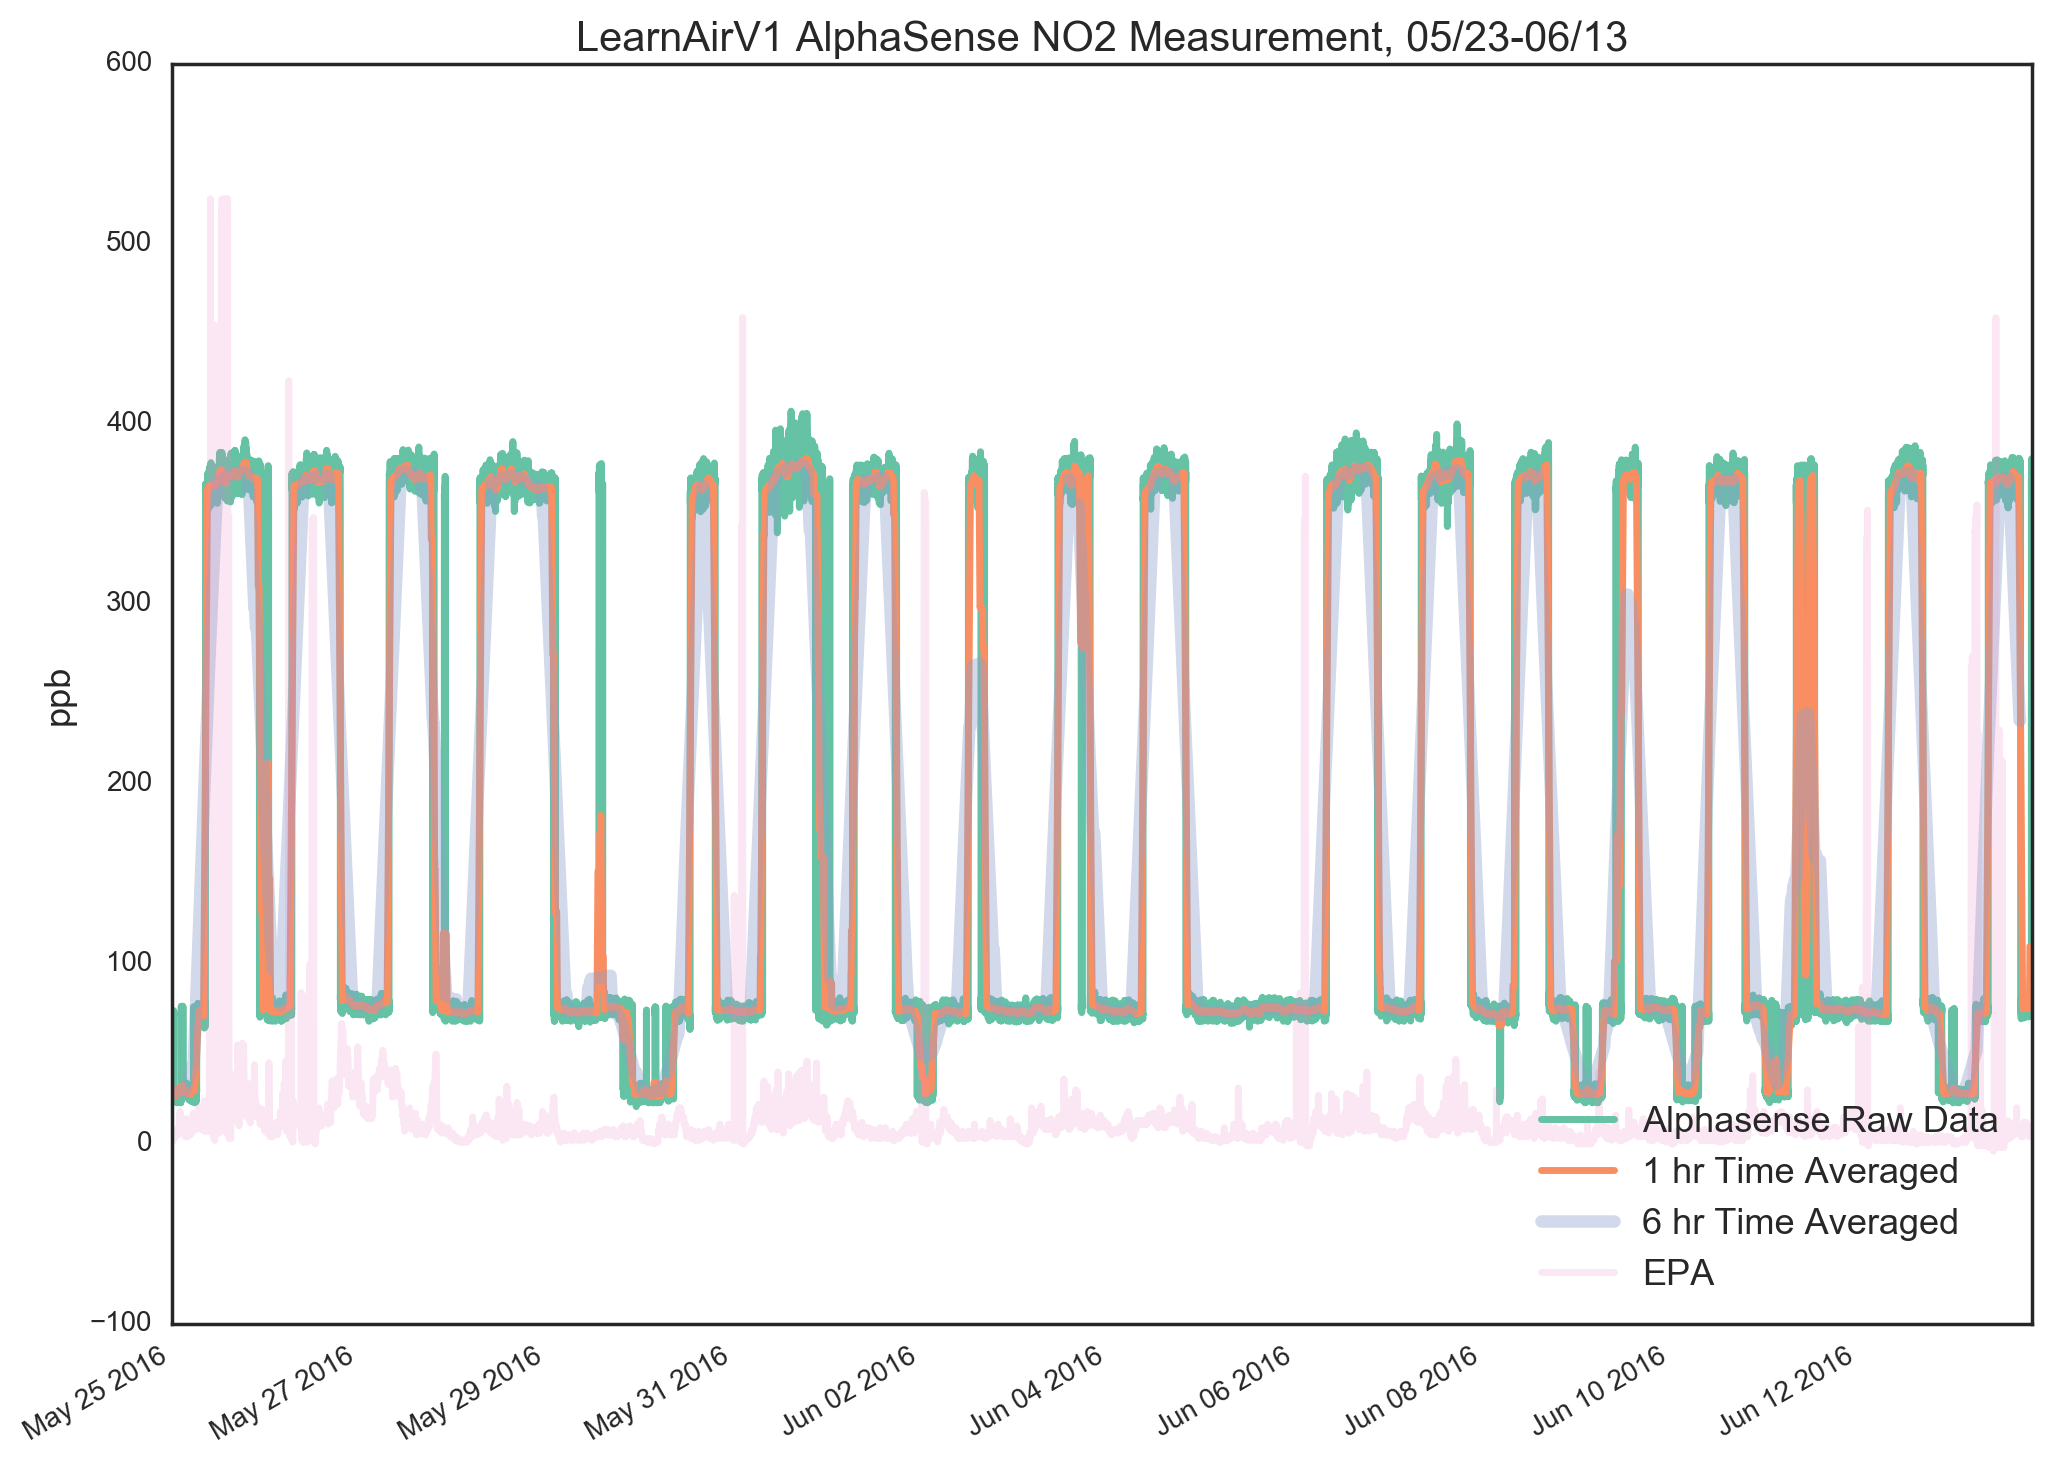
\includegraphics[width=\textwidth]{figs/as_no2_raw}               
 	 \caption{AlphaSense NO2 Raw Data}
  	\label{fig:as_no2_raw}
\end{figure}


\begin{figure}[htb]
 	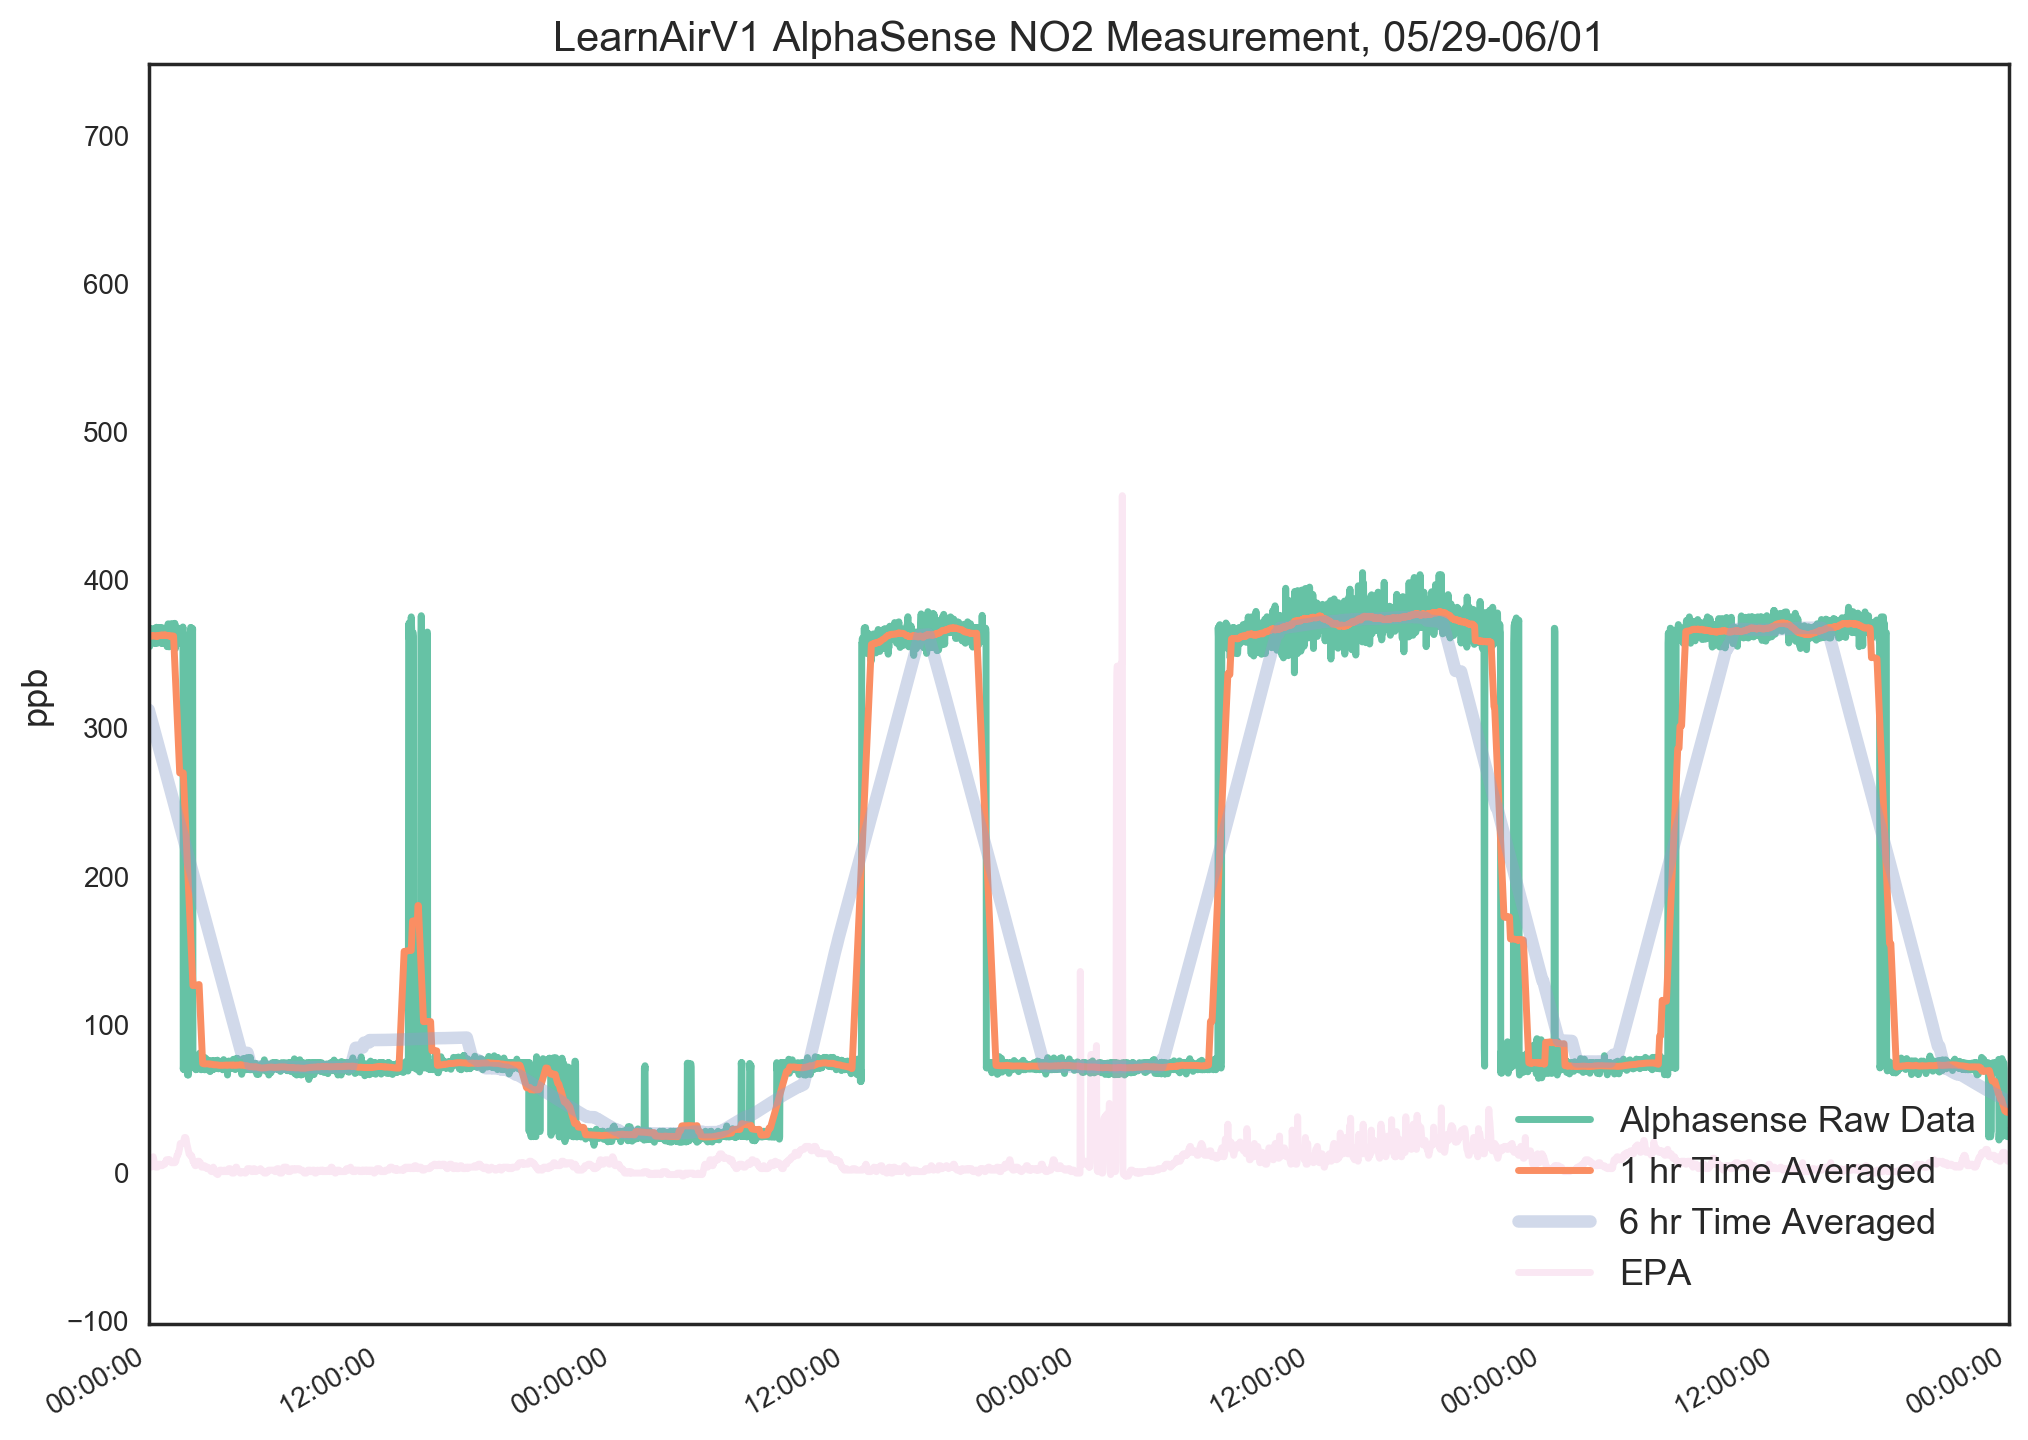
\includegraphics[width=\textwidth]{figs/as_no2_raw_zoomed}               
 	 \caption{AlphaSense NO2 Raw Data Zoomed}
  	\label{fig:as_no2_raw_zoomed}
\end{figure}



\begin{figure}[htb]
 	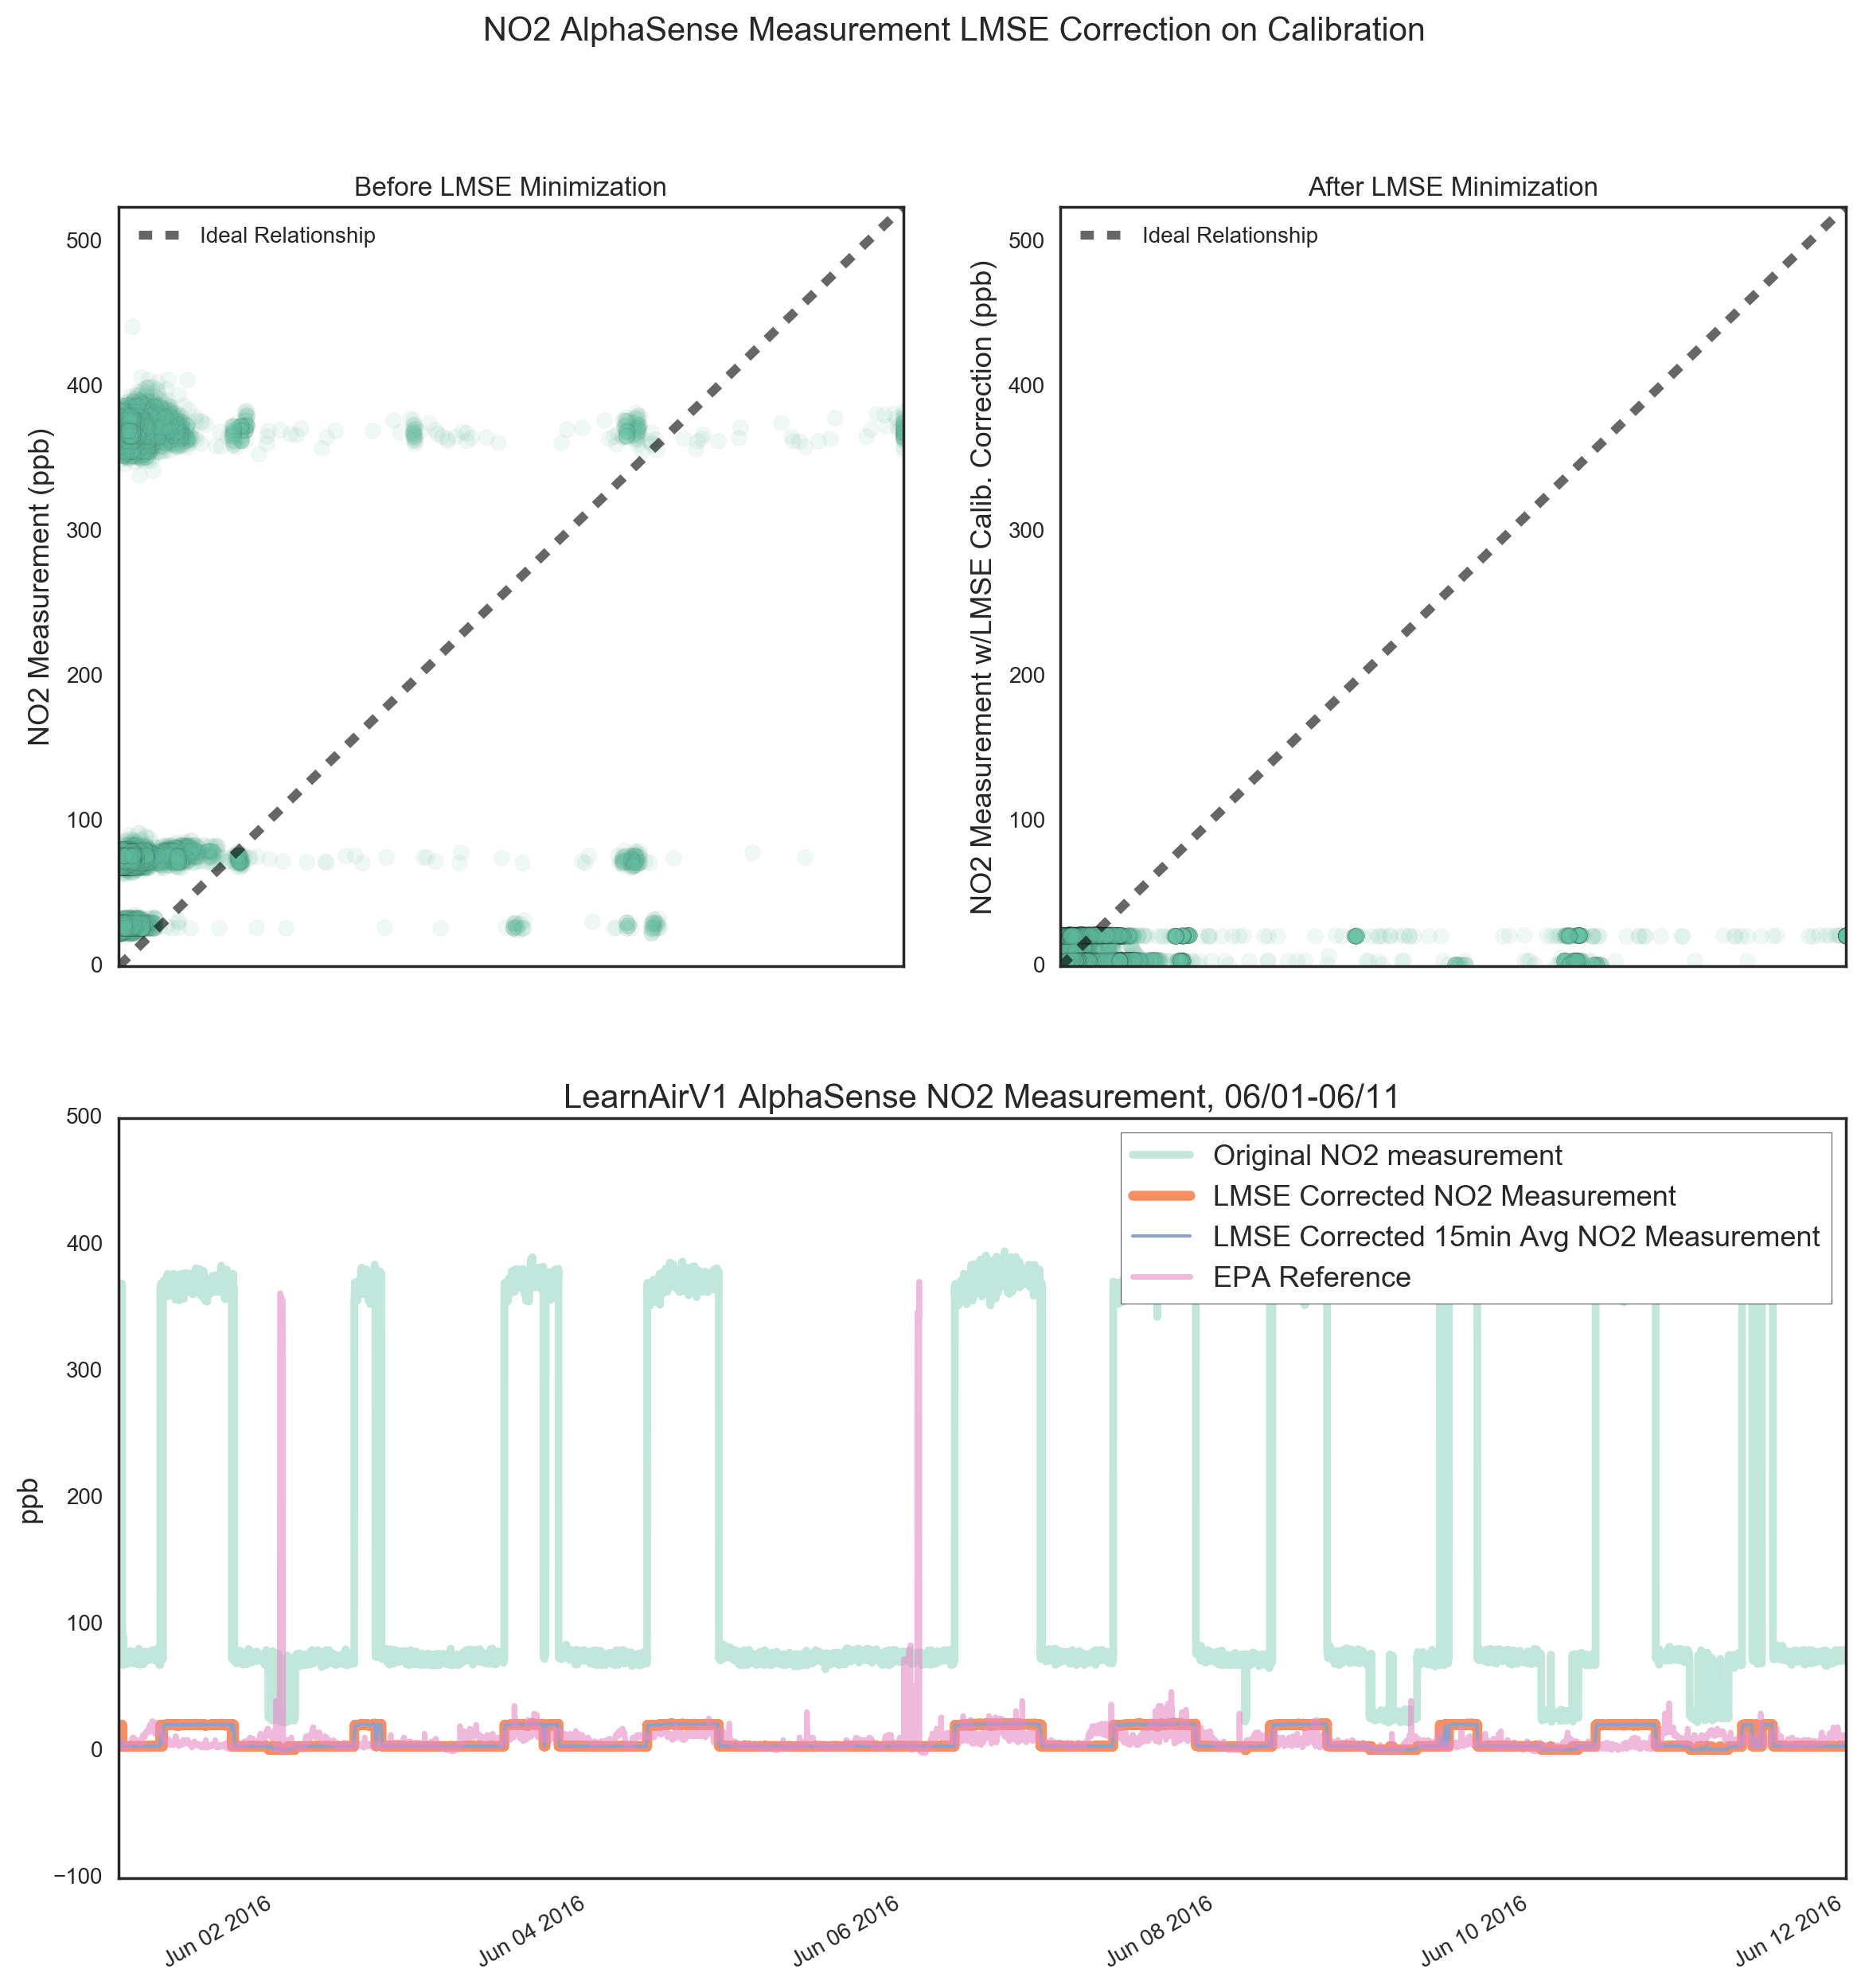
\includegraphics[width=\textwidth]{figs/as_no2_lmse}               
 	 \caption{AlphaSense NO2 after LMSE Calibration}
  	\label{fig:as_no2_lmse}
\end{figure}








\subsection{Machine Learning}


\begin{figure}[htb]
 	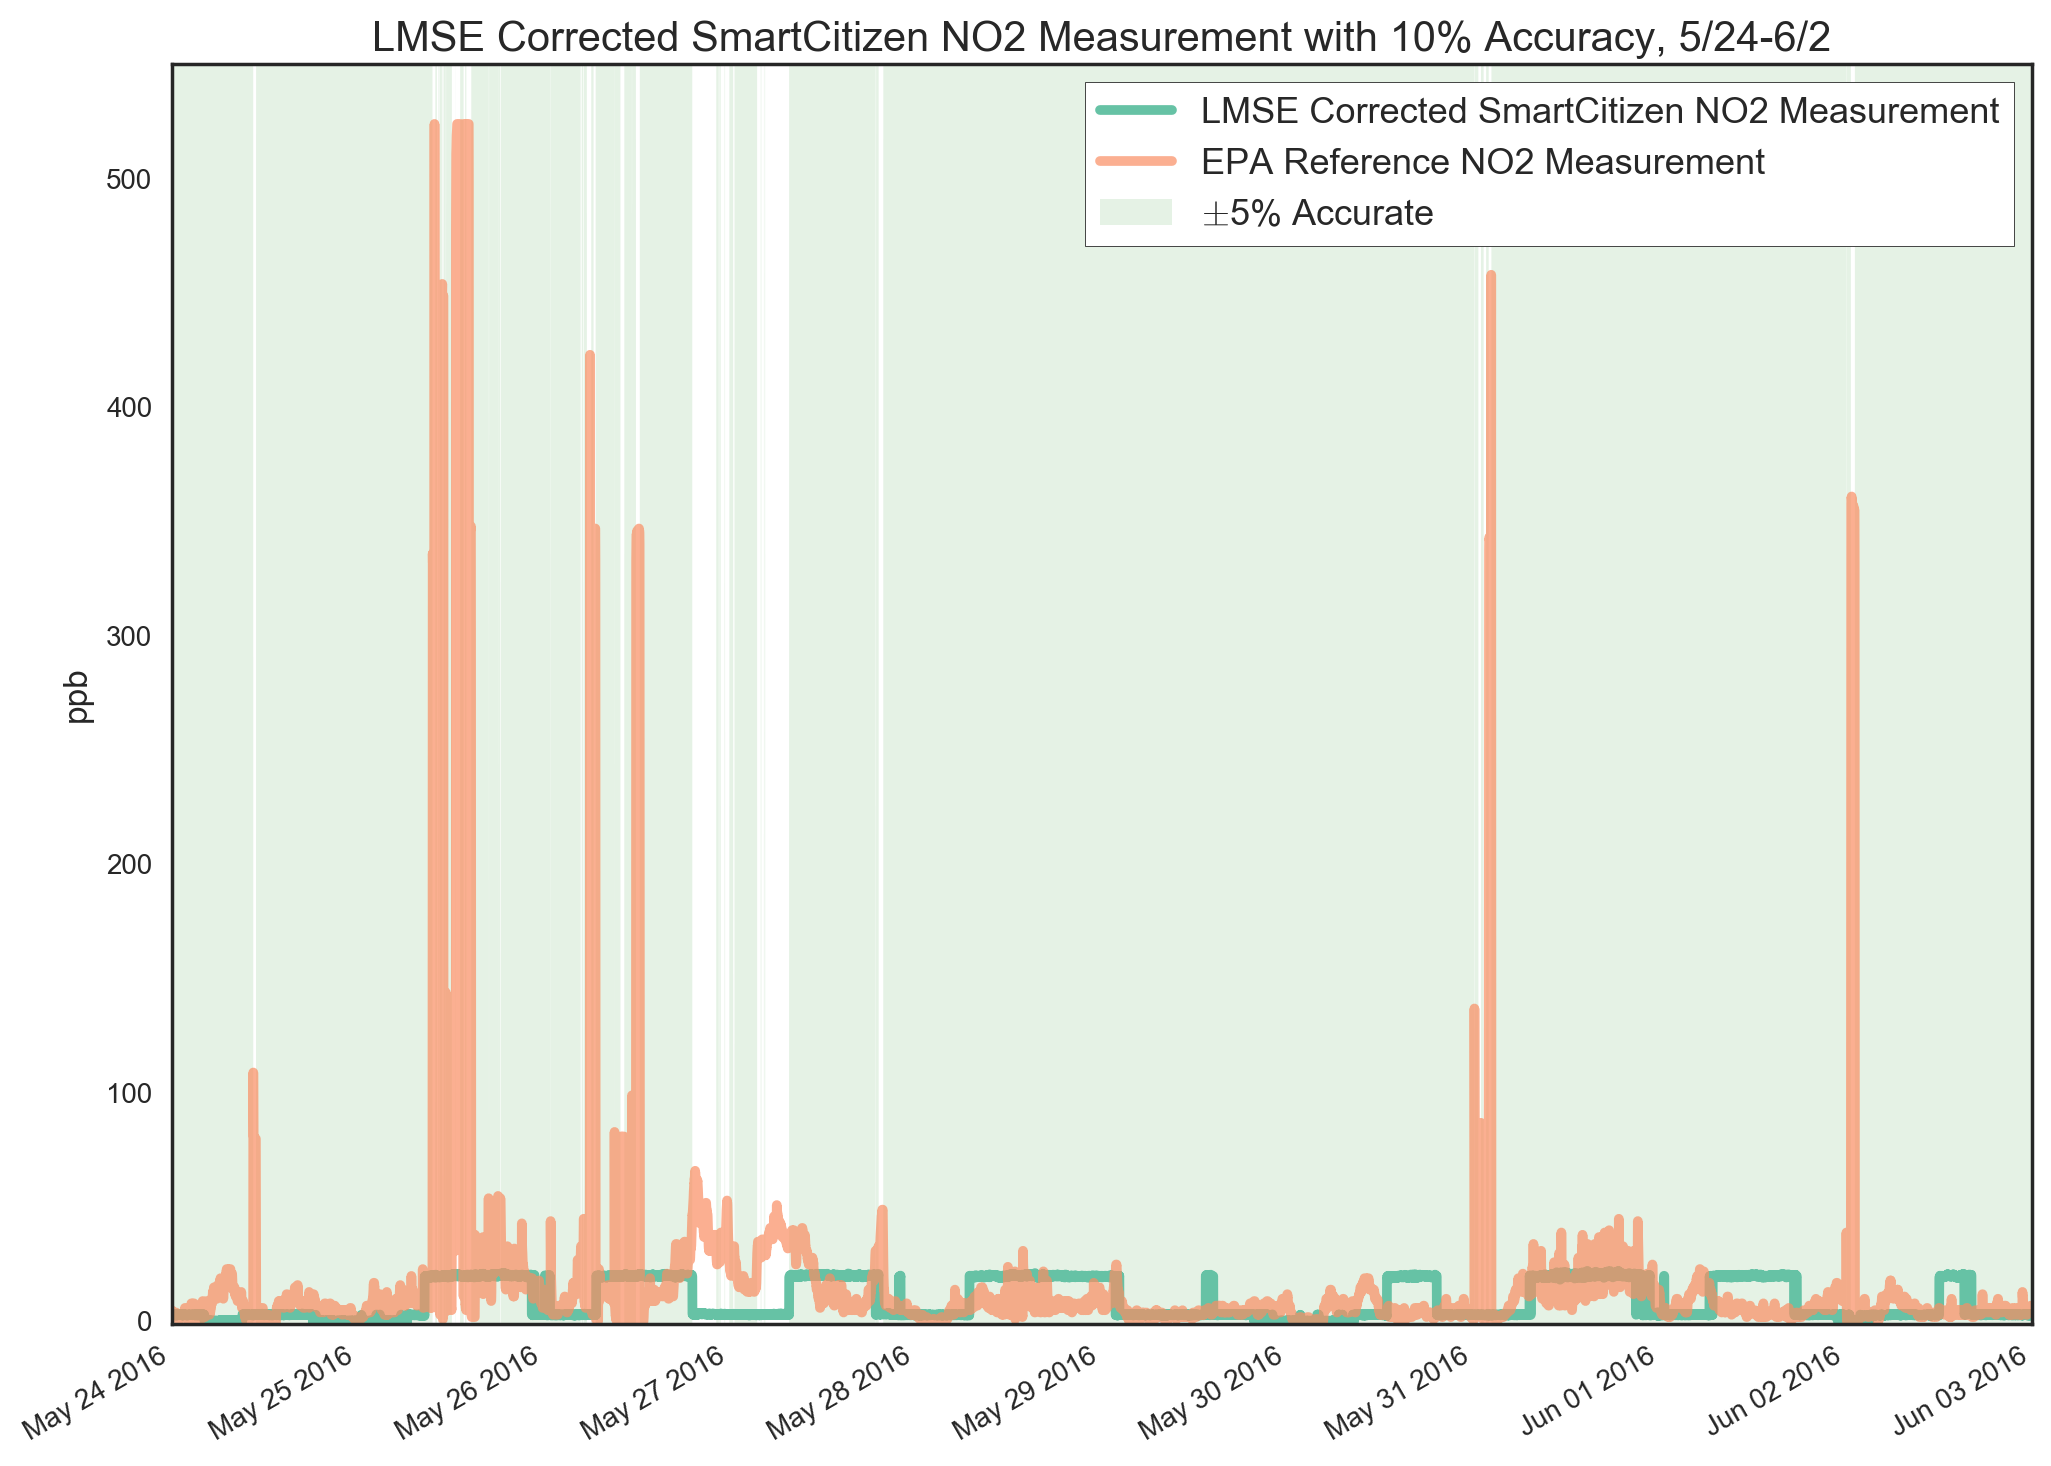
\includegraphics[width=\textwidth]{figs/as_no2_with_10_accuracy_zoomed}               
 	 \caption{AlphaSense NO2 with 10\% Accuracy Threshold}
  	\label{fig:as_no2_with_10_accuracy_zoomed}
\end{figure}

\begin{figure}[htb]
 	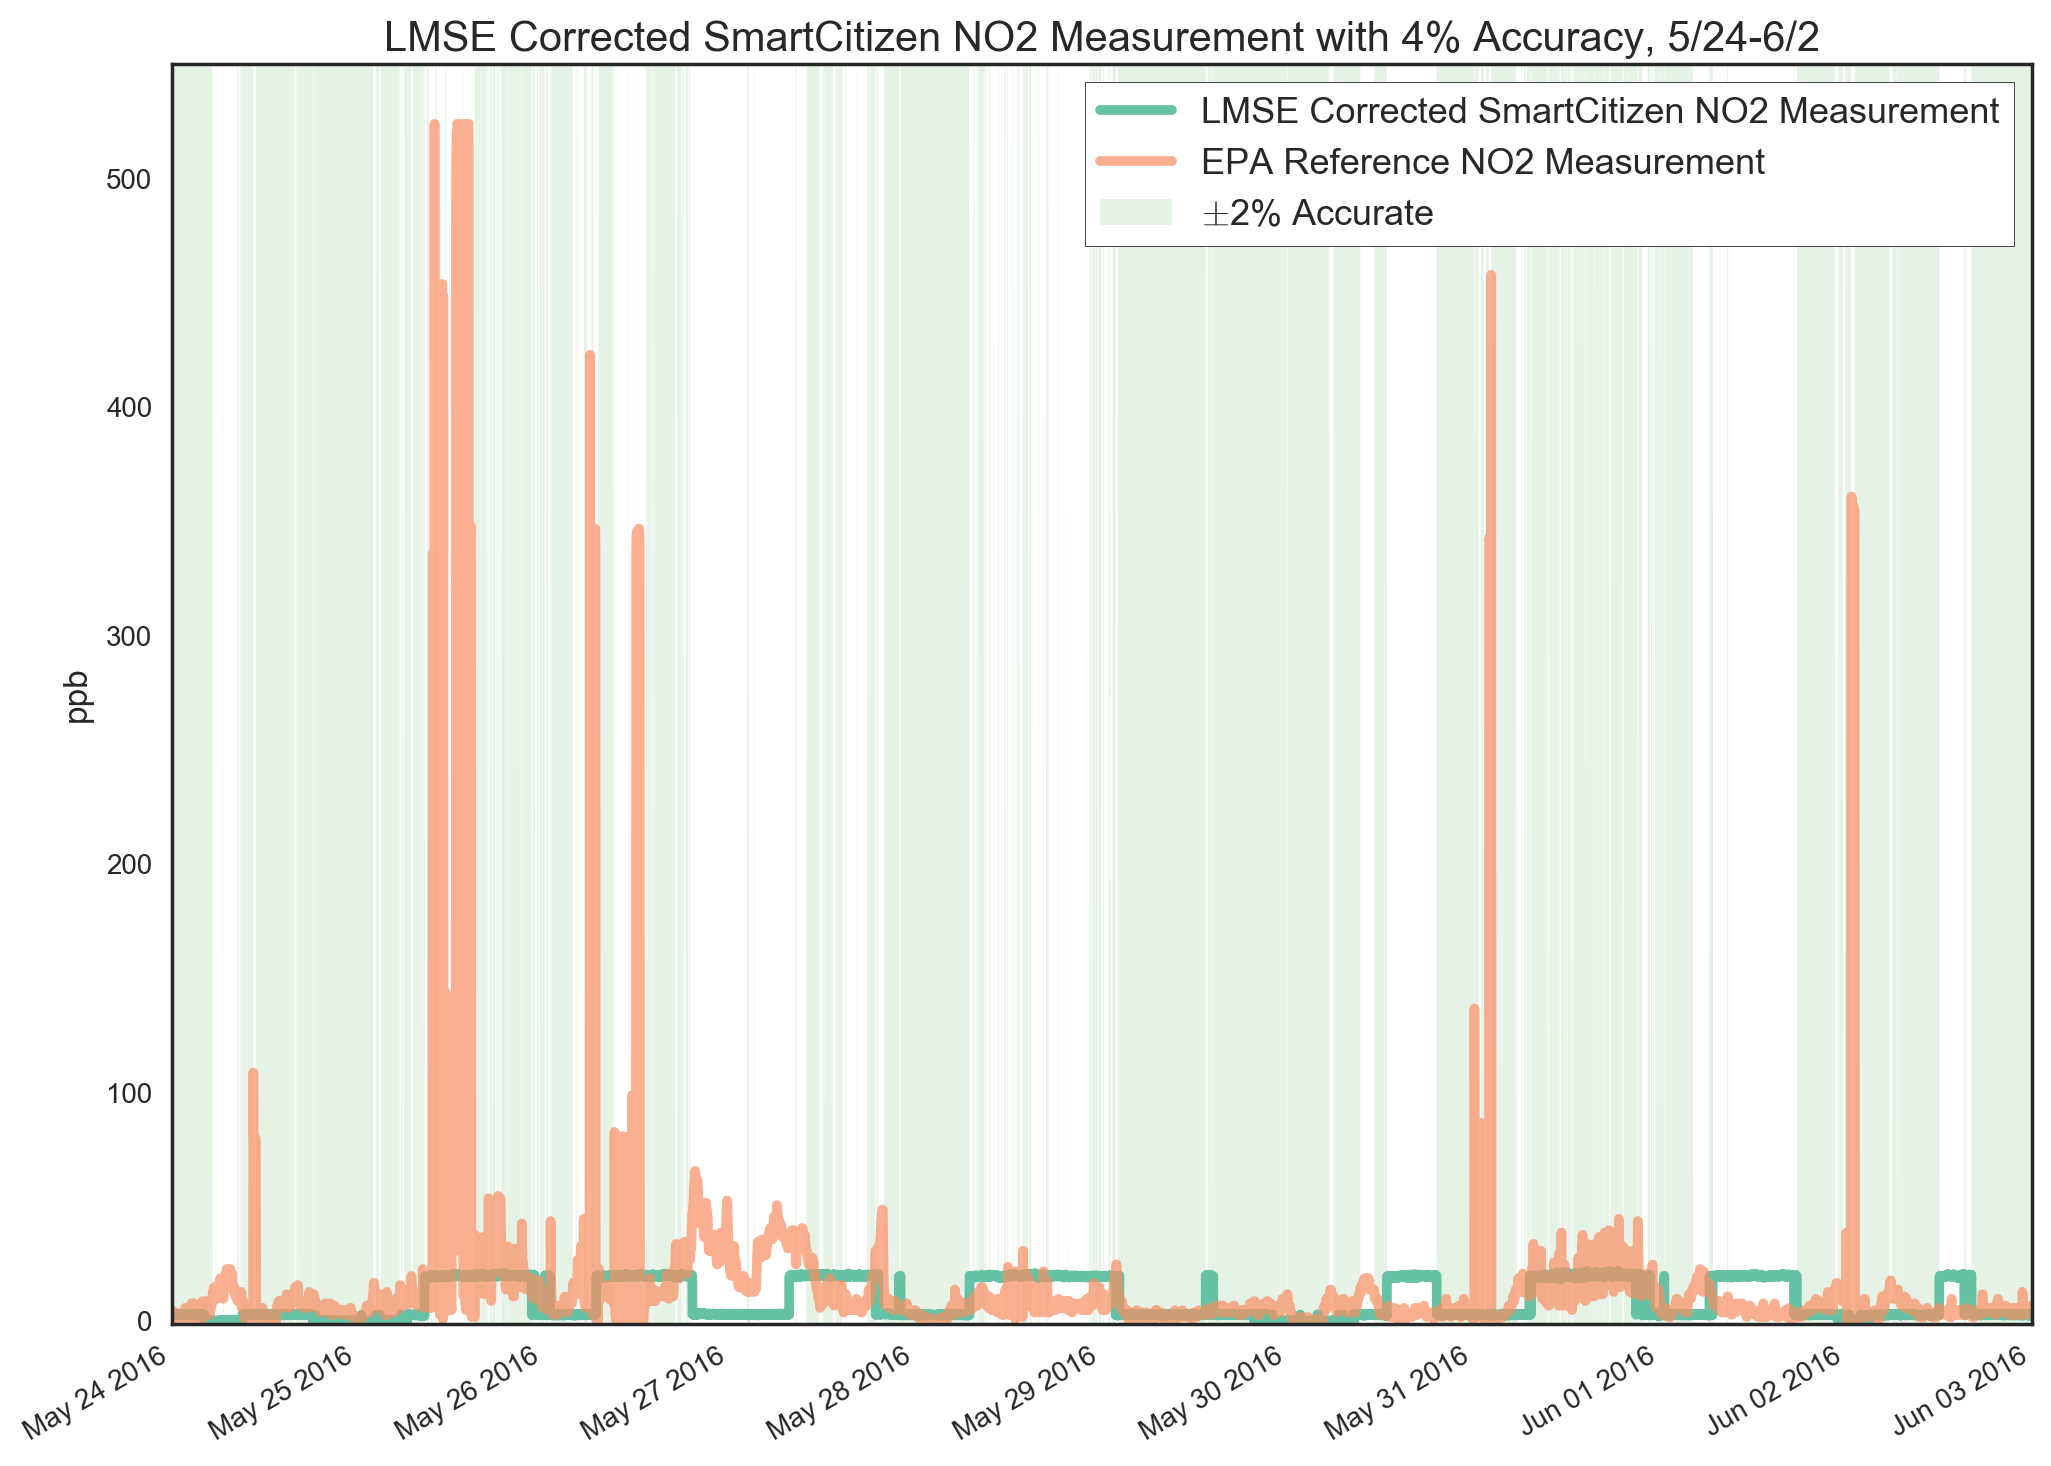
\includegraphics[width=\textwidth]{figs/as_no2_with_4_accuracy_zoomed}               
 	 \caption{AlphaSense NO2 with 4\% Accuracy Threshold}
  	\label{fig:as_no2_with_4_accuracy_zoomed}
\end{figure}




%%%%

parameters = {'C':[0.001, 0.1, 10, 1000], 'penalty':('L1', 'L2') }

===== best ROC\_AUC score 0.961586556822

===== best params {'penalty': 'L1', 'C': 1000}



\begin{table}[H]
\centering
\begin{tabular}{|c|c|c|c|c|}
\toprule
\multicolumn{5}{|c|}{Error Rates for AlphaSense NO2 with Logistic Regression} \\
&\multicolumn{2}{|c|}{all features} & \multicolumn{2}{|c|}{top 15 features} \\
&shuffled & chunked & shuffled & chunked \\
avg & 0.03 & 0.06 & 0.04 & 0.04 \\
min & 0.03 & 0.05 & 0.03 & 0.01 \\
max & 0.03 & 0.14 & 0.04 & 0.14 \\
\bottomrule
\end{tabular}
\label{tab:as1_co_error_rates}
\caption{Error Rates for Predicting AlphaSense NO2 Accuracy with Logistic Regression}
\end{table}



\begin{table}[H]
\centering
\offinterlineskip
\hspace*{-5cm}\raisebox{-3.5cm}[0pt][0pt]{\rotatebox[origin=c]{90}{\parbox[c][0pt][c]{3cm}{\textbf{Actual Values}\\[20pt]}}}\par
\hspace*{1cm}\MyHBox[\dimexpr5.1cm+6\fboxsep\relax]{Predicted Values}\par
\hspace*{1cm}\MyHBox{0}\MyHBox{1}\par
\MyTBox{0}{116.2}{130.2}
\MyTBox{1}{34.0}{5749.6}
}
\label{tab:as_no2_confusion}
\caption{Average AlphaSense NO2 Confusion Matrix w/Shuffled K-Fold}
\end{table}


\begin{figure}[htb]
 	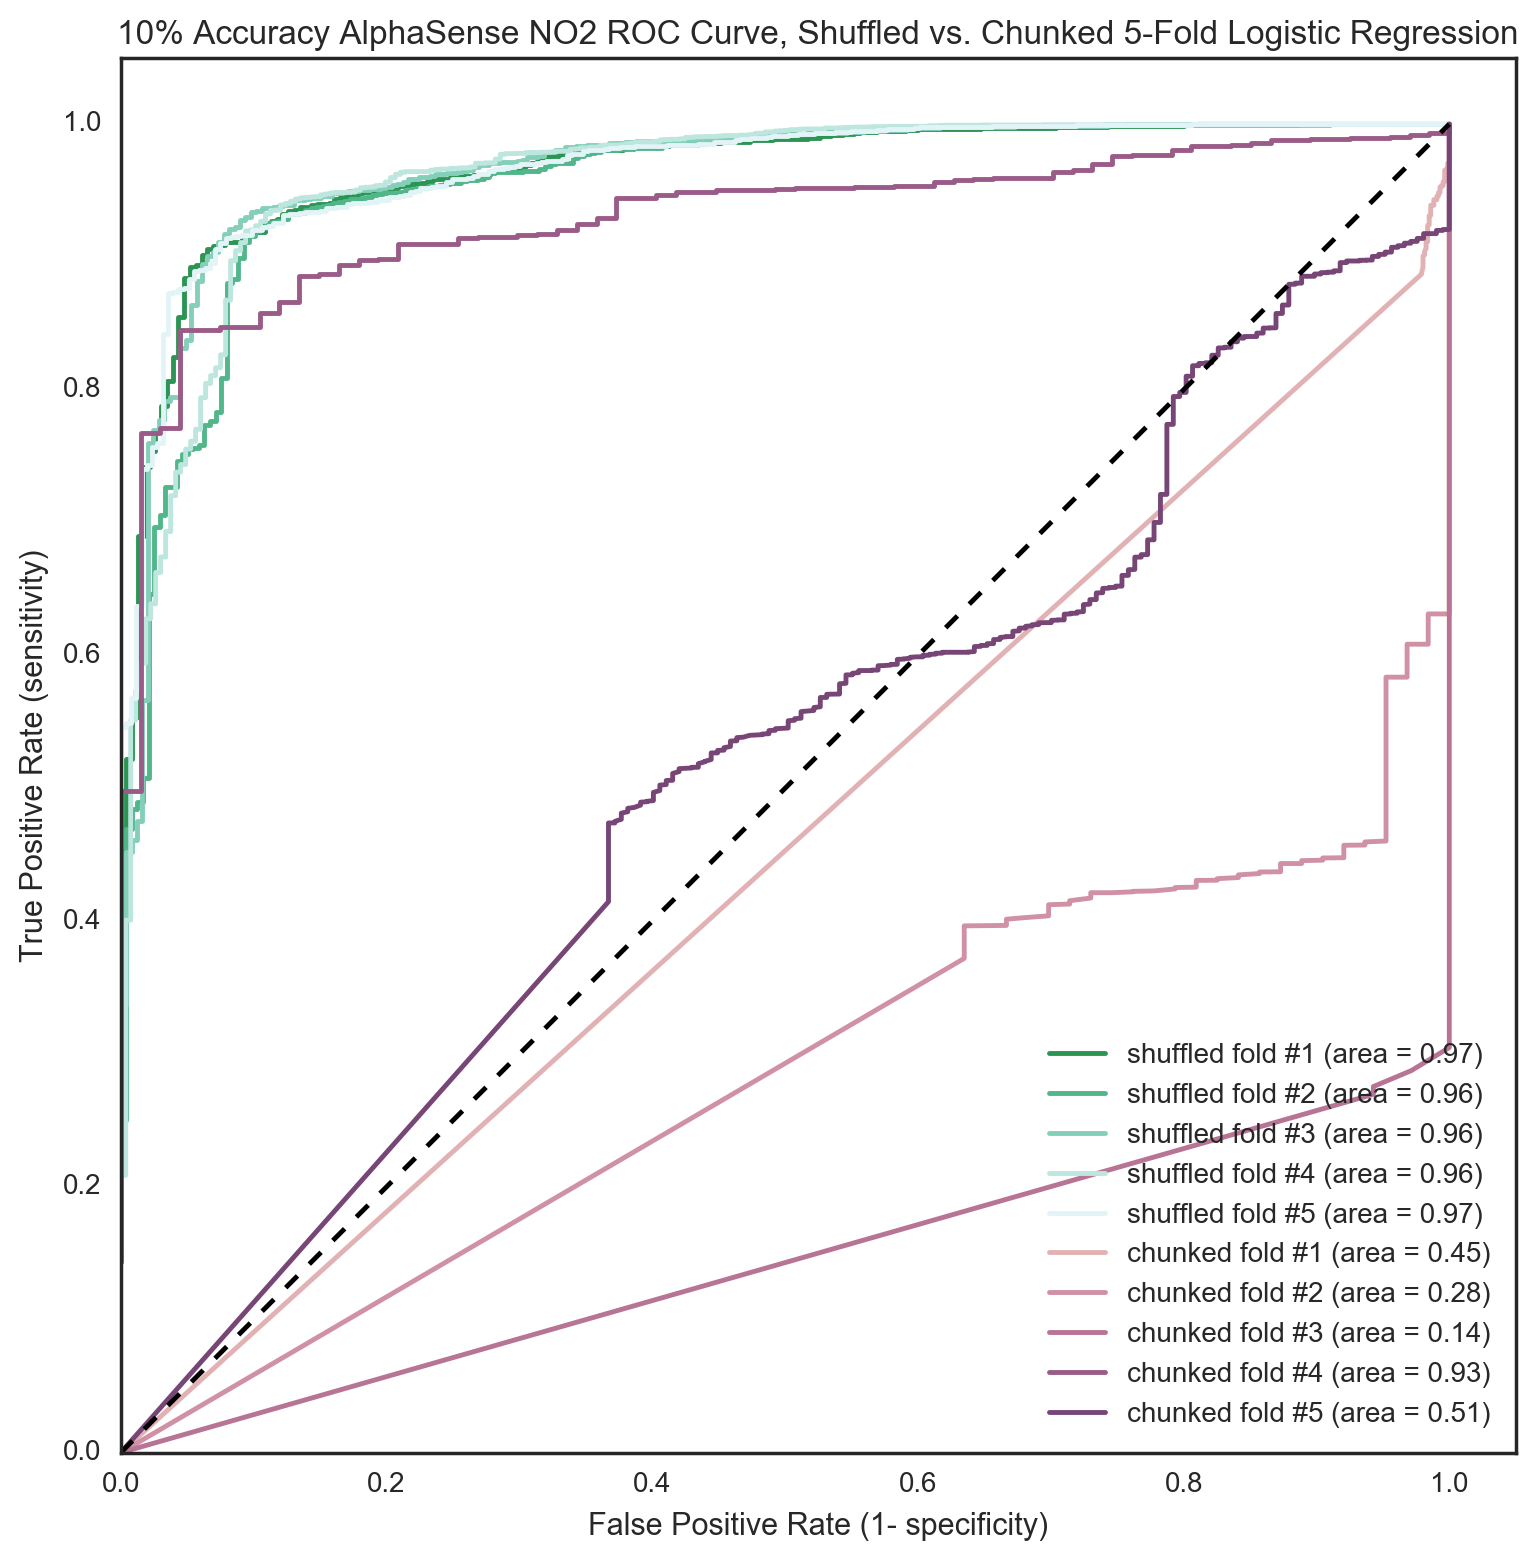
\includegraphics[width=\textwidth]{figs/as_no2_10_roc}               
 	 \caption{AlphaSense NO2 ROC Curve}
  	\label{fig:as_no2_10_roc}
\end{figure}


here's text referencing the (Table \ref{tab:as_no2_randomforest_features}).

\begin{table}[H]
\centering
\begin{tabular}{lllllllll}
\\
\\
\toprule
Feature & Importance \\
\midrule
 avg\_60\_bkcarbon & 0.0422524706607 \\
 avg\_1440\_bkcarbon & 0.0417472204692 \\
 bkcarbon & 0.0385594210158 \\
 avg\_720\_bkcarbon & 0.0347584125412 \\
 min\_since\_plugged\_in & 0.0203302045169 \\
 avg\_60\_forecastio\_windSpeed & 0.0164269542704 \\
 derivative\_avg\_1440\_bkcarbon & 0.0162252088513 \\
 avg\_60\_forecastio\_windBearing & 0.0159723111776 \\
 avg\_1440\_lmse\_calib\_as\_co & 0.0149001557286 \\
 avg\_720\_lmse\_scaled\_sharpDust & 0.0148211173957 \\
 day\_of\_year & 0.0145567862081 \\
 avg\_60\_forecastio\_pressure & 0.0142569975814 \\
 daily\_avg\_sck\_humidity & 0.013849933762 \\
 avg\_30\_ws & 0.0137791673751 \\
 daily\_avg\_forecastio\_temperature & 0.0136871069105 \\
\bottomrule
\end{tabular}
\label{tab:as_no2_randomforest_features}
\caption{Top 15 Features from Random Forest for AlphaSense NO2, used in Pruned Logistic Regression}
\end{table}



\begin{figure}[htb]
 	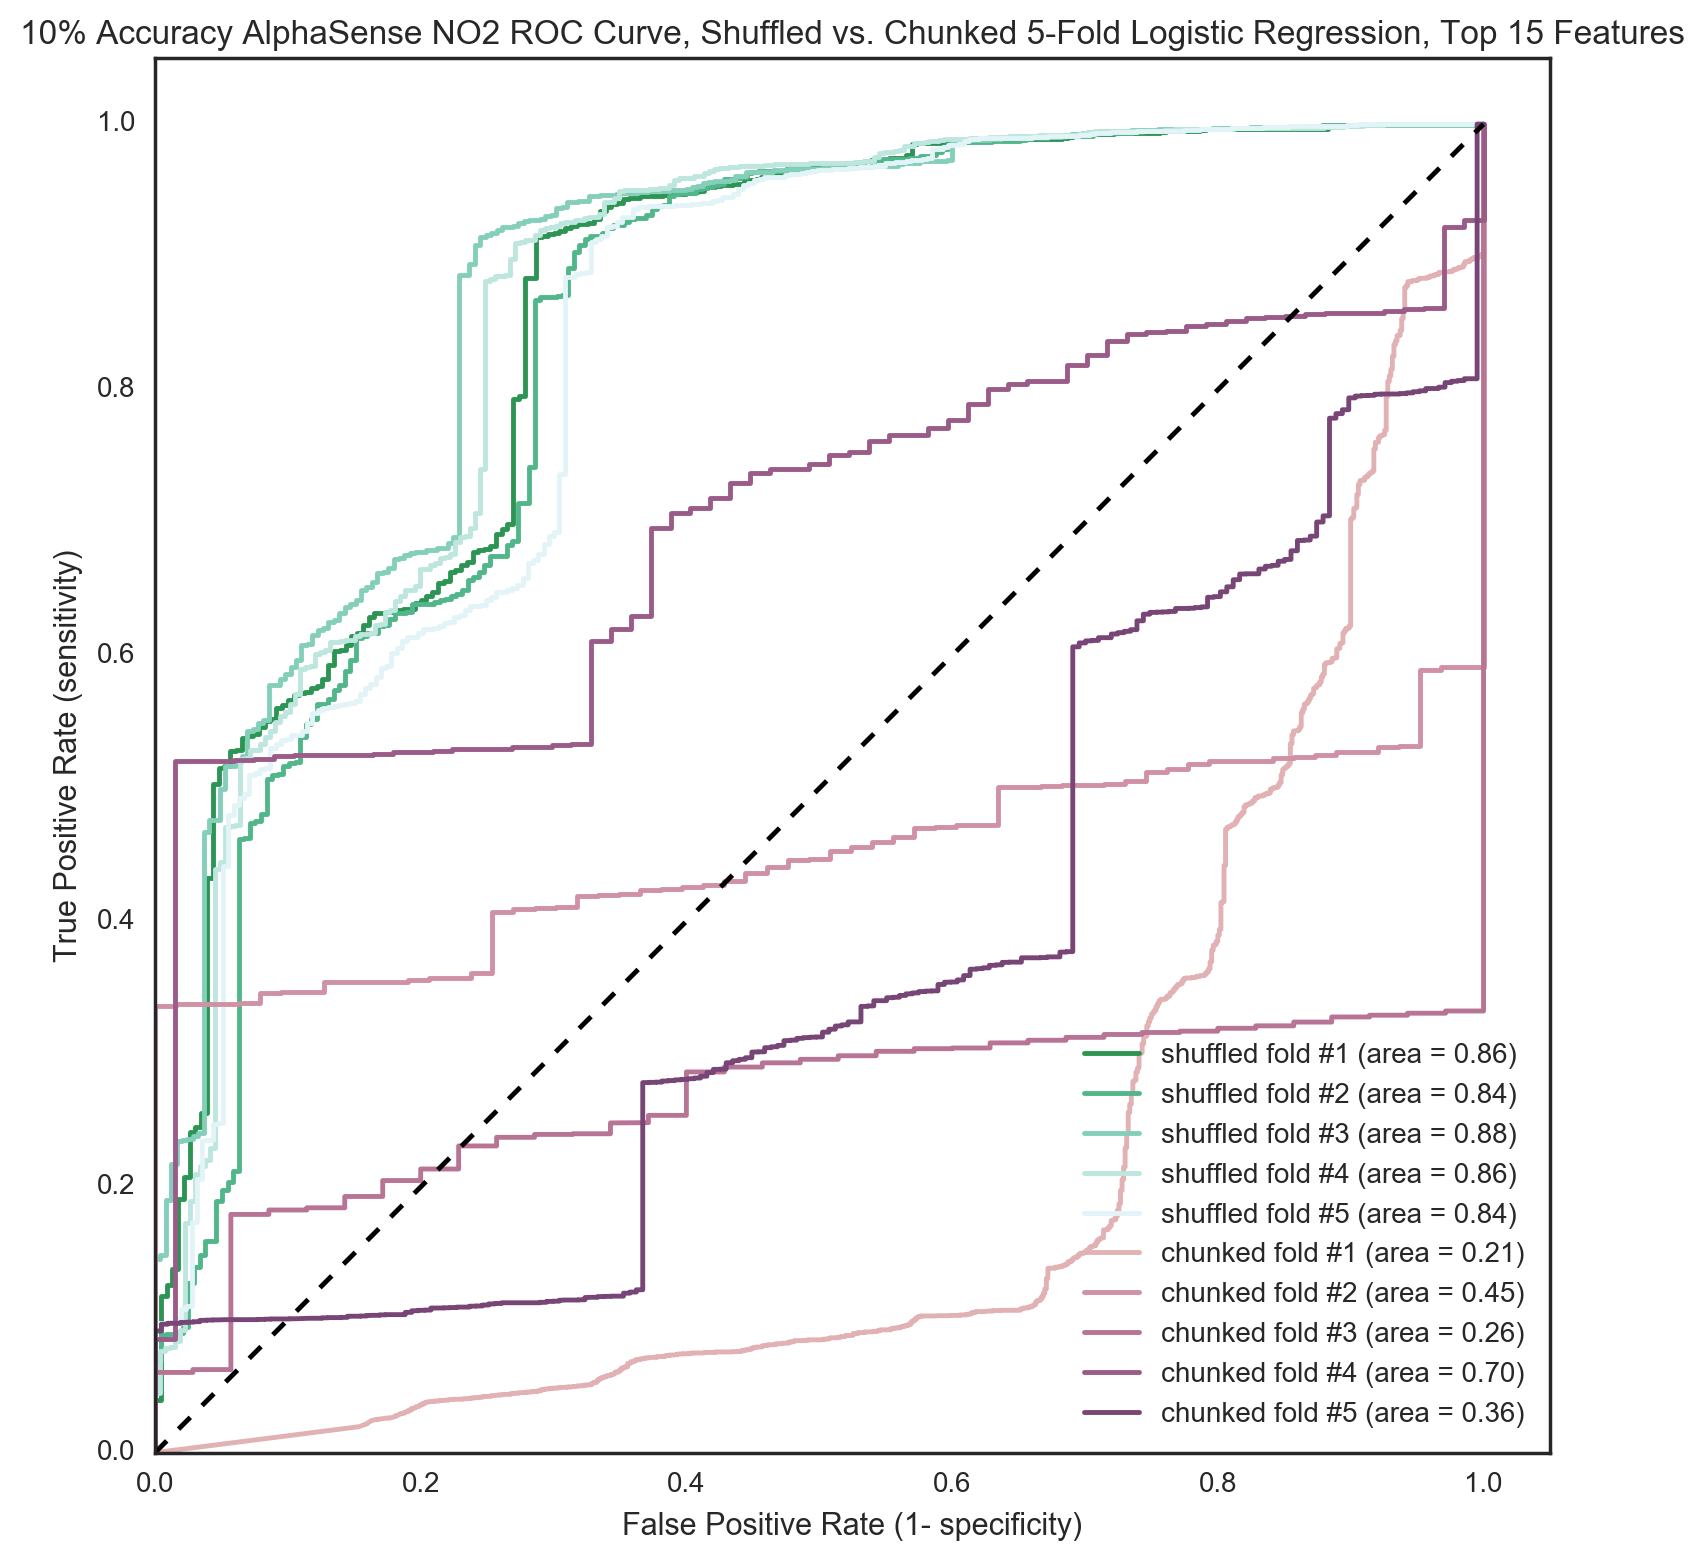
\includegraphics[width=\textwidth]{figs/as_no2_10_roc_pruned_features}               
 	 \caption{AlphaSense NO2 ROC Using Top 15 Features}
  	\label{fig:as_no2_10_roc_pruned_features}
\end{figure}

\begin{figure}[htb]
 	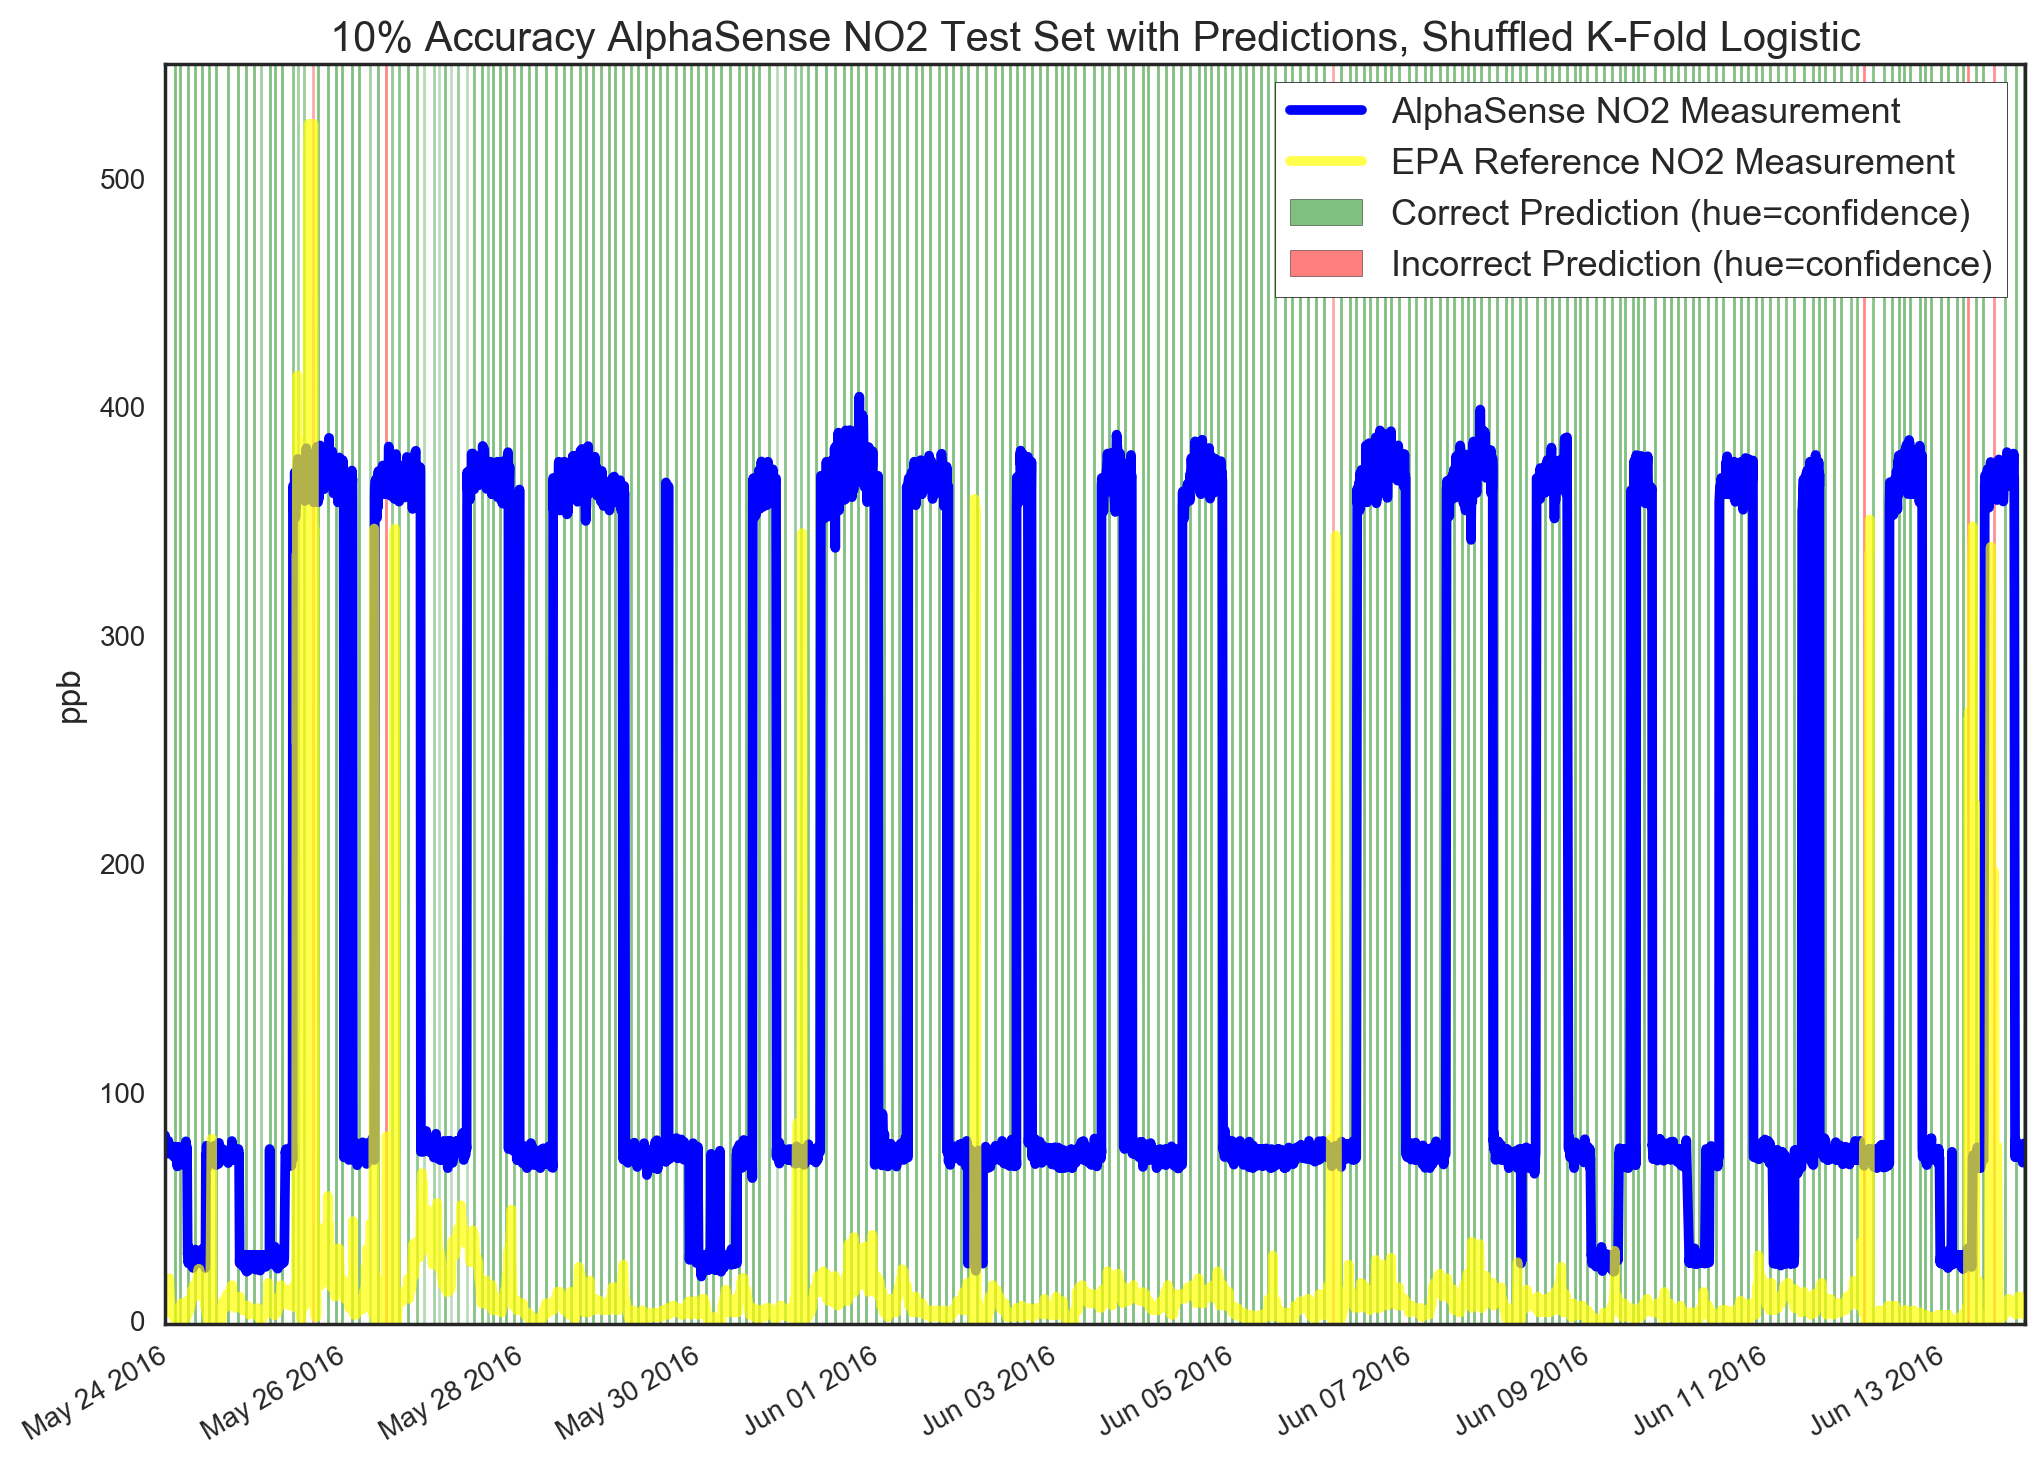
\includegraphics[width=\textwidth]{figs/as_no2_10_logistic_predictions}               
 	 \caption{AlphaSense NO2 Prediction Accuracy}
  	\label{fig:as_no2_10_logistic_predictions}
\end{figure}



here's text referencing the (Table \ref{tab:as_no2_top_features}).

\begin{table}[H]
\centering
\begin{tabular}{lllllllll}
\\
\\
\toprule
     & Corr. & Lasso & Lin Reg & RF   & RFE  & Ridge & Stability & Mean \\
\midrule
bkcarbon                          & 0.99  & 0     & 0          & 0.85 & 0.47 & 0.23  & 0.79      & 0.48 \\
avg\_60\_bkcarbon                 & 1     & 0     & 0          & 1    & 0.54 & 0.14  & 0.64      & 0.47 \\
avg\_1440\_bkcarbon               & 0.9   & 0     & 0          & 0.16 & 0.5  & 0.44  & 0.69      & 0.38 \\
daily\_avg\_sck\_humidity         & 0.36  & 0     & 0          & 0.03 & 0.59 & 0.77  & 0.39      & 0.31 \\
as\_o3                            & 0.02  & 0     & 0          & 0.97 & 0.77 & 0.01  & 0.42      & 0.31 \\
lmse\_sck\_co                     & 0.06  & 1     & 0          & 0.01 & 0.81 & 0     & 0.28      & 0.31 \\
avg\_60\_forecastio\_cloudCover   & 0.16  & 0     & 0          & 0.11 & 0.53 & 0.38  & 0.81      & 0.28 \\
Solar Panel ( V)                  & 0.05  & 0     & 1          & 0    & 0.87 & 0     & 0         & 0.27 \\
derivative\_avg\_1440\_bkcarbon   & 0.17  & 0     & 0          & 0.04 & 0.62 & 0.08  & 1         & 0.27 \\
sck\_humidity\_saturated          & 0.04  & 0     & 0          & 0.01 & 0.58 & 1     & 0         & 0.23 \\
avg\_720\_lmse\_scaled\_sharpDust & 0     & 0     & 0          & 0.37 & 0.57 & 0.67  & 0.01      & 0.23 \\
avg\_720\_bkcarbon                & 0.85  & 0     & 0          & 0.2  & 0.16 & 0.06  & 0.35      & 0.23 \\
evening                           & 0.05  & 0     & 0          & 0    & 0.95 & 0.04  & 0.47      & 0.22 \\
day                               & 0.06  & 0     & 0          & 0    & 0.99 & 0.06  & 0.42      & 0.22 \\
night                             & 0.06  & 0     & 0          & 0    & 1    & 0.06  & 0.41      & 0.22 \\
alphaS2\_work                     & 0.31  & 0.78  & 0          & 0.02 & 0.21 & 0.05  & 0.09      & 0.21 \\
forecastio\_fog                   & 0.05  & 0     & 0.4        & 0    & 0.93 & 0     & 0         & 0.2  \\
forecastio\_temperature\_c        & 0     & 0     & 0.01       & 0    & 0.93 & 0.01  & 0.44      & 0.2  \\
derivative\_avg\_720\_bkcarbon    & 0.09  & 0     & 0          & 0.05 & 0.61 & 0.15  & 0.5       & 0.2  \\
forecastio\_temperature           & 0     & 0     & 0          & 0    & 0.92 & 0.01  & 0.41      & 0.19 \\
Carbon Monxide ( kOhm)            & 0.06  & 0     & 0          & 0.01 & 0.82 & 0     & 0.34      & 0.18 \\
forecastio\_cloudCover            & 0.19  & 0     & 0          & 0.01 & 0.44 & 0.17  & 0.48      & 0.18 \\
forecastio\_partly-cloudy-day     & 0.05  & 0     & 0.04       & 0    & 0.89 & 0.01  & 0.23      & 0.17 \\
\bottomrule
\end{tabular}
\label{tab:as_no2_top_features}
\caption{Top Features for Predicting AlphaSense NO2}
\end{table}
